\section{Struktura projektu}

\vspace{0.5cm}
\begin{figure}[ht]
    \centering
    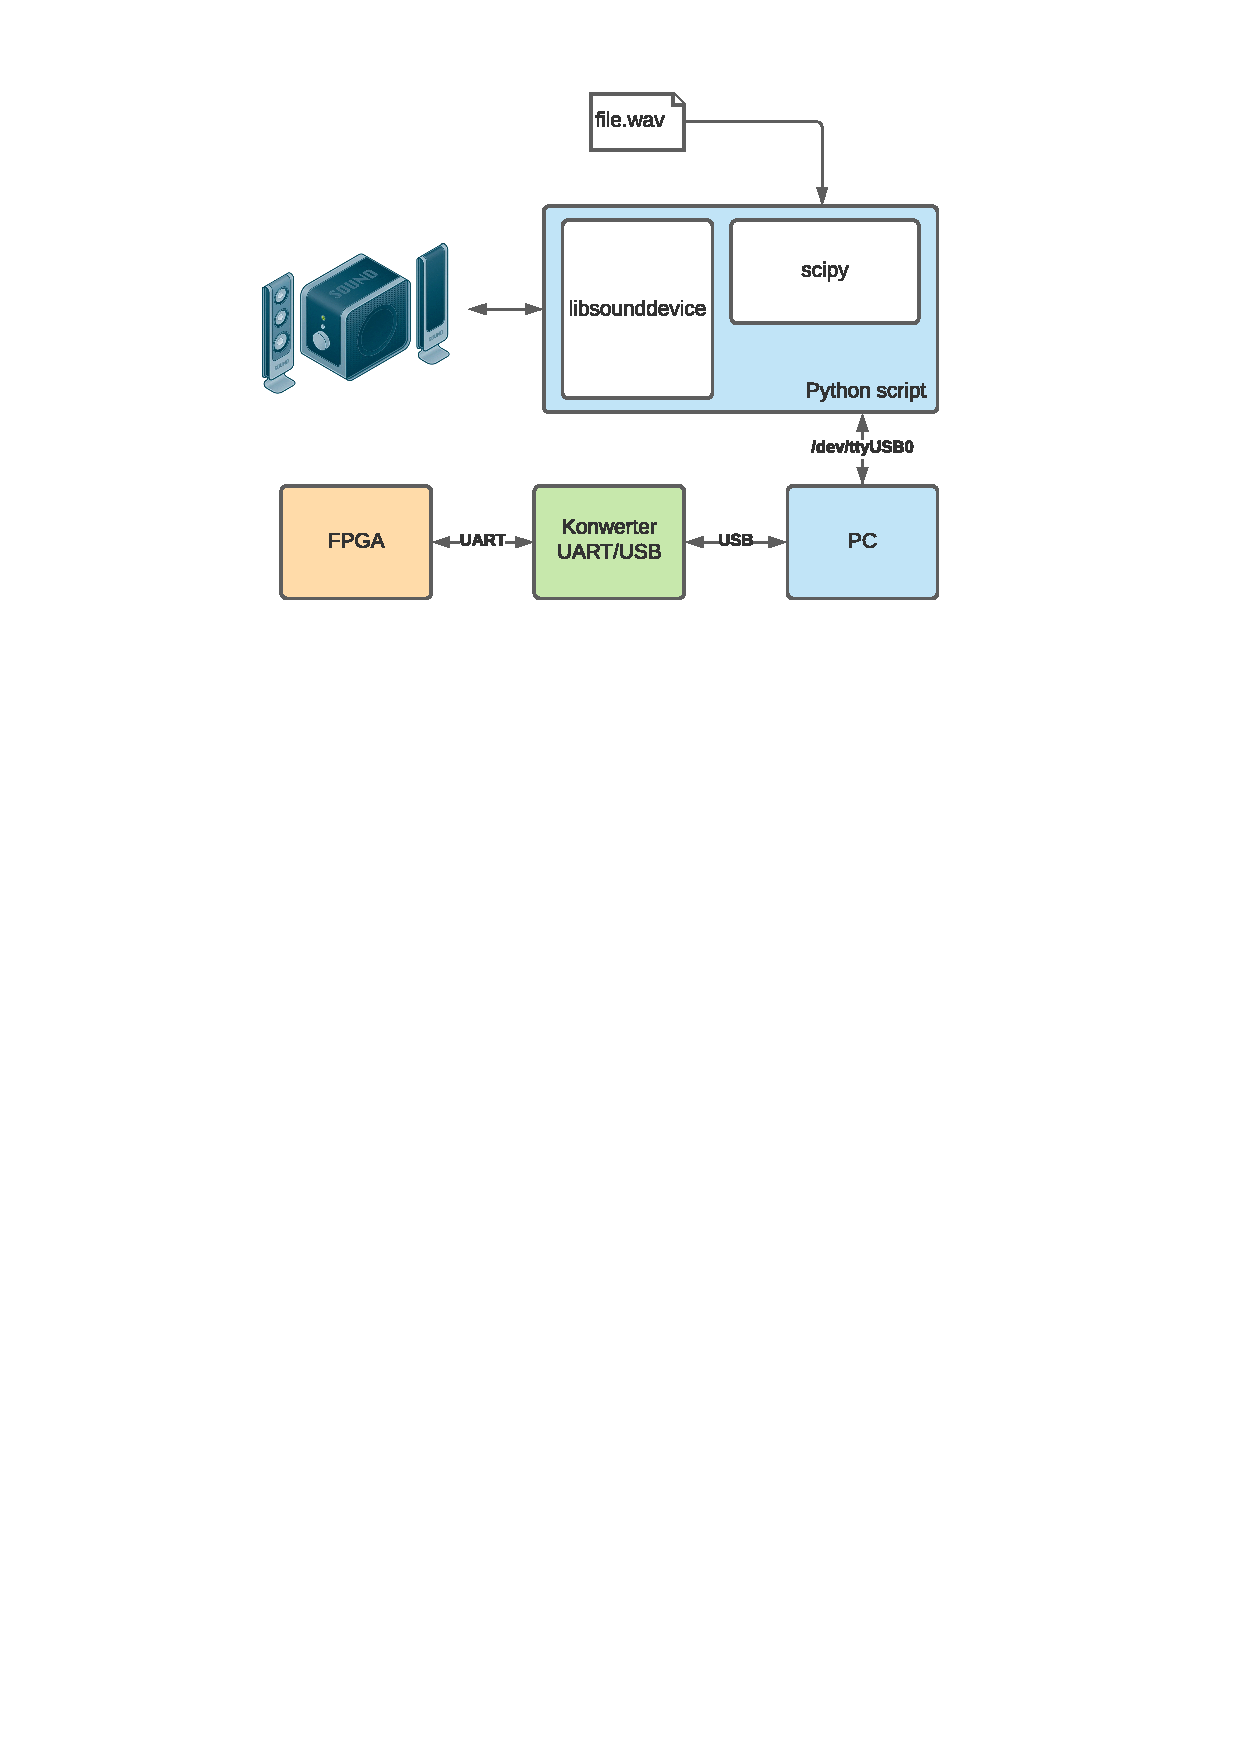
\includegraphics[scale=0.75]{img/diagrams/system.pdf}
    \captionsetup{format=plain,justification=centering}
    \caption{Struktura systemowa projektu}
    \label{system-structure}
\end{figure}
\vspace{0.5cm}

Realizację przedstawionej w~części pierwszej koncepcji rozpoczęto od nakreślenia struktury projektu na trzech płaszczyznach: \textbf{systemowej}, \textbf{implementacyjnej} i~\textbf{projektowej}. Pierwsza z~nich obejmowała zdefiniowanie węzłów, które będą brały udział w~procesie przetwarzania dźwięku od otwarcia zawierajacego go pliku do chwili wyemitowania przetworzonej wersji przez urządzenie audio. Jak przedstawiono na Rys. \ref{system-structure}, wyróżniono cztery zasadnicze jednostki. \textit{Skrypt języka Python} odpowiedzialny jest za załadowanie pliku dźwiękowego do pamięci RAM, przekazanie i~odebranie go z~układu przetwarzającego, a~także wysterowanie domyślnego urządzeni audio w~oparciu o~zmodyfikowane próbki. Urządzeniem przetwarzającym jest oczywiście układ \textit{FPGA}, który implementuje wymienione wyżej filtry. Pośrednikami w~komunikacji pomiędzy układem scalonym a~aplikacją są oparty o~układ FT232R \textit{mostek USB/UART} oraz \textit{komputer klasy PC}. Taka konfiguracja pozwala na dwukierunkową transmisję danych z~prędkością do 375KB na sekundę, co przy założeniu 16-bitowych próbek oraz częstotliwości próbkowania na poziomie 44100Hz powinno wystarczyć do strumieniowania dźwięku zarówno w~trybie mono jak i~stereo. W~projekcie wykorzystano biblioteki \verb|sounddevice| oraz \verb|scipy| języka Python. Pierwsza z~nich udostępnia interfejs dla szerokiej gamy urządzeń audio, natomiast druga pozwala przetwarzać pliki w~formacie WAV do postaci tablic danych biblioteki \verb|numpy|. Aby zredukować czas wykonywania operacji na wirtualnym porcie szeregowym, zdecydowano się podzielić strumieniowane dane na bloki o~wielkości 5000B, które wysyłane są do układu FPGA pojedynczo.

Określenie struktury implementacyjnej obejmowało doprecyzowanie zaproponowanych w~części pierwszej koncepcji konfiguracji urządzenia. Ostatecznie zdecydowano się na model przedstawiony na Rys. \ref{fpga-structure}. Wyróżnić w~nim można cztery zasadnicze części. Odbiornik oraz nadajnik UART zostały wcielone w~ramy dwóch szerszych struktur, które umożliwiają wymianę N-bajtowych próbek danych w~ramach pojedynczej transakcji. W~ramach interfejsu użytkownika wykorzystano moduł XADC (ang. \textit{Xilinx Analog/Digital Converter}), który w~ramach jednostki \verb|AnalogScanner| pozwala konwertować sekwencję do 16 sygnałów analogowych podłączonych do układu poprzez zewnętrzny multiplekser. Umożliwi to dołączenie szeregu potencjometrów odpowiedzialnych za określanie parametrów filtrów przedstawionych w~centralnej części rysunku. Aby zmaksymalizować elastyczność konfiguracji postanowiono pozostać przy pierwotnej koncepcji jednolitego interfejsu efektów, którego szczegóły zostaną omówione w~dalszej części dokumentu. Dodatkowym elementem konfiguracji jest także zestaw rejestrów konfiguracyjnych, które określają porametry interfejsów komunikacyjnych oraz sposób mapowania mierzonych wartości analogowych na parametry filtrów. Na ten moment zostały one zaimplementowane w~sposób niejawny, jednak w~przyszłości planowane jest zmiana tego podejścia na rzecz ułatwienia rekonfiguracji urządzenia.

\vspace{0.5cm}
\begin{figure}[ht]
    \centering
    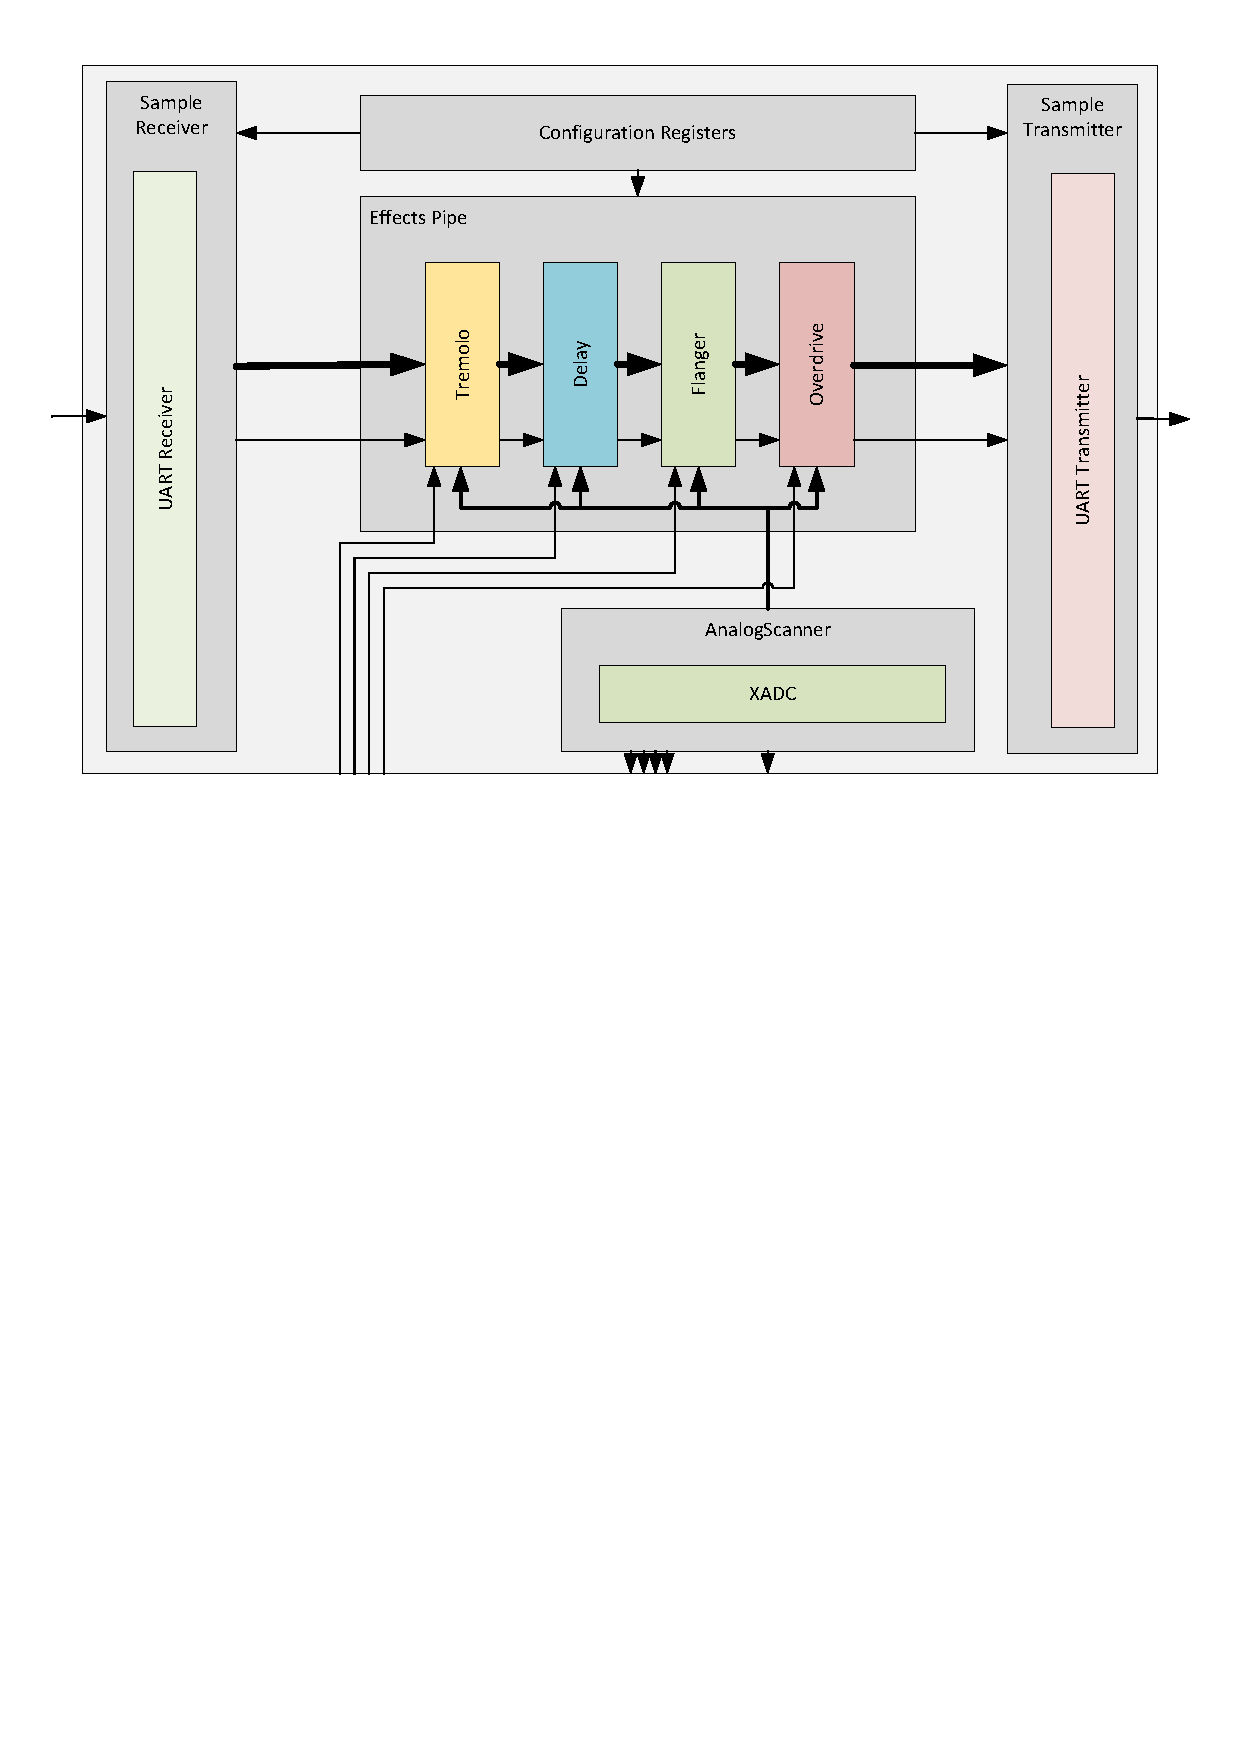
\includegraphics[scale=0.75]{img/diagrams/project_diagram.pdf}
    \captionsetup{format=plain,justification=centering}
    \caption{Struktura implementacyjna projektu}
    \label{fpga-structure}
\end{figure}
\vspace{0.5cm}

Ostatnią - choć nie mniej ważną z~perspektywy projektanta - kwestią wymagającą określenia była struktura samego projektu rozumiana jako podział drzewa plików i~katalogów. Oprogramowanie \textit{Vivado} wykorzystywane na etapie symulacji oraz syntezy nie jest w~opinii autora optymalnym środowiskiem programistycznym\footnote{Vivado jest oczywiście środowiskiem służącym do \textbf{konfiguracji} a~nie programowania układów FPGA. Z~uwagi na brak lepszego terminu postanowiono jednak pozostać przy określeniu \textit{środowisko programistyczne}}. Elementami, które składają się na taki stan rzeczy są m.in. męczący oczy interfejs graficzny oraz brak integracji z~systemami kontroli wersji. Z~tego względu zdecydowano się na wykorzystanie oprogramowania \textit{Visual Studio Code} jako domyślnego narzędzia tworzenia kodu oraz zarządzania projektem. Aby było to możliwe koniecznym stało się zapoznanie się z~odpowiednimi dokumentami (\cite{vivado_design_flow}, \cite{vivado_design_methodology}) udostępnianymi przez firmę Xilinx. Pozwoliło to określić te z~plików generowanych przez \textit{Vivado}, które są konieczne do odtworzenia struktury projektu. Na tej podstawie zdecydowano się na podział przedstawiony na Rys. \ref{project-structure}. Elementami wartymi wyróżnienia są katalogi \textit{src/ip} oraz \textit{workdir}. Pierwszy z~nich przechowuje pliki w~formacie XML opisujące konfigurację wykorzystywanych w~projekcie bloków XADC oraz BRAM (ang. \textit{Block Random Access Memory}), które zostały wyekstrahowane ze struktury projektowej \textit{Vivado}. Drugi stanowi z~kolei miejsce docelowe dla hierarchii plików generowenj przez samo oprogramowanie. Jedynym jej elementem, który włączony został do systemu kontroli wersji jest plik \verb|GuitarMultieffect.xpr| zawierający pełny opis struktury projetktu. Warto zauważyć, że przyjęte podejście do kontroli wersji pozwoli na uruchomienie projektu jedynie przy użyciu aktualnie wykorzystywanej wersji \textit{Vivado} (2020.2).

\vspace{0.5cm}
\begin{figure}[ht]
    \centering
    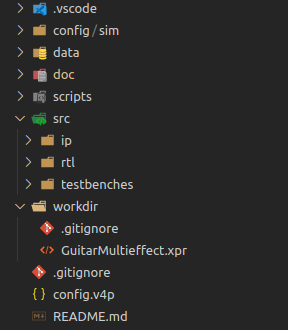
\includegraphics[scale=0.7]{img/source_structure.png}
    \captionsetup{format=plain,justification=centering}
    \caption{Struktura projektowa}
    \label{project-structure}
\end{figure}
\vspace{0.5cm}
